\pagestyle{fancy}
\fancyhf{}
\rhead{\rightmark}
\lhead{\thepage}

\chapter{Hamiltonian systems and Symplectic structure}
In this chapter we are going to introduce some important concepts regarding dynamical systems and how they relate to Hamiltonian systems and its geometric structure. Also we describe the theory involving the numerical integration of differential equations conserving the symplectic structure. These descriptions are made mostly following Ref. \cite{ott_chaos_2002} and Ref. \cite{sanz2018numerical}.





\section{Dynamical systems}
Generally speaking, a dynamical system may be defined as set of deterministic mathematical equations whose solution shows how the system evolves in time. Time may be taken as a continuous or a discrete variable. A typical example of a dynamical system that adopts time as a parameter varying in  a continuous way is a system of $n$ first order, autonomous, ordinary differential equations,

%\begin{align}
\begin{eqnarray} 
\frac{dx^{(1)}}{dt}&=F_1(x^{(1)},x^{(2)},...,x^{(n)}),\nonumber \\
\frac{dx^{(2)}}{dt}&=F_2(x^{(1)},x^{(2)},...,x^{(n)}),\\
&\vdots \nonumber \\
\frac{dx^{(n)}}{dt}&=F_n(x^{(1)},x^{(2)},...,x^{(n)}),
\nonumber
\label{eq:set_diff_eqs}
\end{eqnarray} 
%\end{align}
we can rewrite this set of equations by adopting a notation for a compact equation using the vector form of equations

\begin{equation}
\frac{d\vec{x}(t)}{dt}=\vec{F}[\vec{x}(t)],
\label{eq_:vect_diff_eqs}
\end{equation}

here we take $\vec{x}$ as an $n$ dimensional vector that represents the state of the system at a given time $t$ and $\vec{F}$ is a function depending on the variable $\vec{x}$. This set of equations represent a dynamical system, for an initial state given by $\vec{x}(0)$, it is possible in principle to be able to solve this set of equations in time and retrieve the state $\vec{x}(t)$ of the system for any given $t>0$. The figure (\ref{fig:3d_orbit_ps}) shows the points followed as the system evolves in time for the case of $n=3$. The space $(x^{(1)},x^{(2)}x^{(3)}$ in the figure is more known as the phase space, and the path in the phase space is referred as orbit or trajectory. When we speak of dynamical systems using continuous time, it is common to refer to these orbits as a flow.

\begin{figure}[H]
\centering
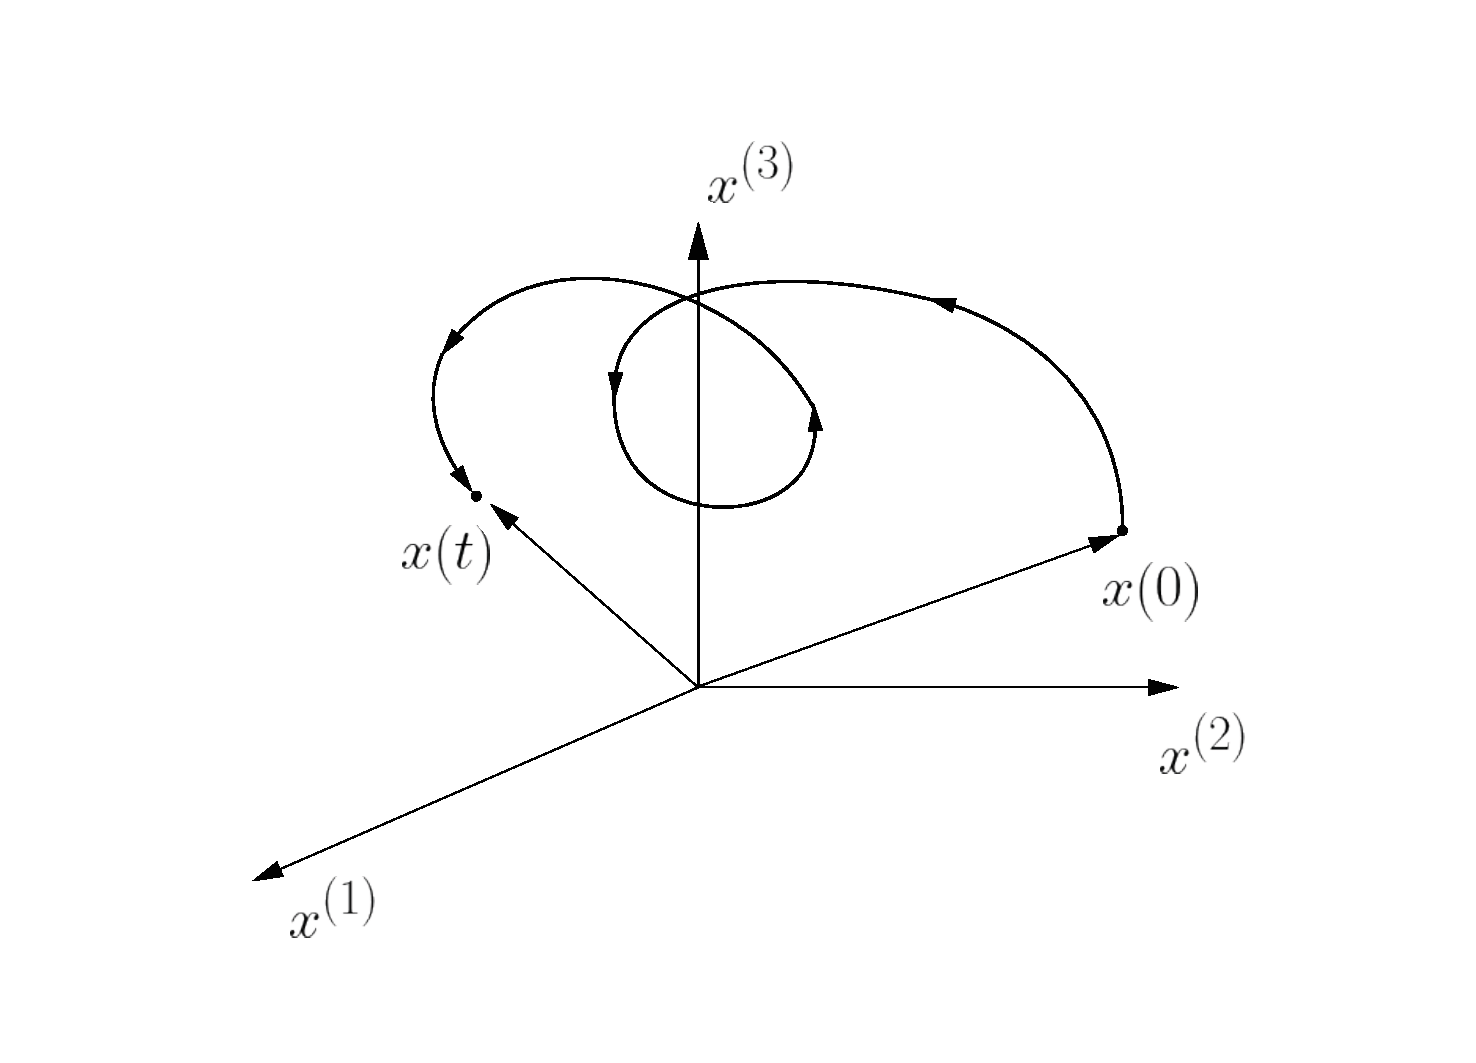
\includegraphics[width=1.\textwidth]{Figures/orbit_3d.pdf}
\caption{Orbit in three dimensional phase space}
\label{fig:3d_orbit_ps}
\end{figure}

For the case of discrete systems, time is represented as integer values ($t=1,2,3,...$). The best example of a dynamical system with discrete time is a map, which can be written in vector notation as
\begin{equation}
\vec{x} _{t+1}=\vec{M}(\vec{x}_t),
\label{eq:discrete_dyn_sys}
\end{equation}

where $\vec{x}_t$ is an n-dimensional vector $\vec{x}_t=(x^{1}_t,x^{2}_t,...,x^{n}_t)$ and $\vec{M}$ a function of $\vec{x}_t$. Given an initial state $\vec{x}_0$, it is possible to obtain the state at time $t=1$ by applying the map $\vec{x}_{1}=\vec{M}(\vec{x}_0)$. Having determined $\vec{x}_1$ it will be possible to determine the state at time $t=2$ by applying the map again but to the new state at $t=1$ as $\vec{x}_2=\vec{M}(\vec{x}_1)$ and so on. Thus, given an initial condition $\vec{x}_0$ we generate a trajectory of the discrete time system in time: $\vec{x}_0,\vec{x}_1,\vec{x}_2,...$. 

A dynamical system that posses continuous time evolution may be reduced to a discrete time system to evaluate in more detail the dynamical properties of the differential equaitions by using the technique called Poincaré Surface Section. To do so we consider a set of $n$ first order, autonomous, ordinary differential equations such as in  (\ref{eq:set_diff_eqs}), a Poincaré map represents a reduction of the flow in the n-dimensional space to a map of dimension $n-1$. To illustrate this, an example with $n=3$ is given:

\begin{figure}[H]
\centering
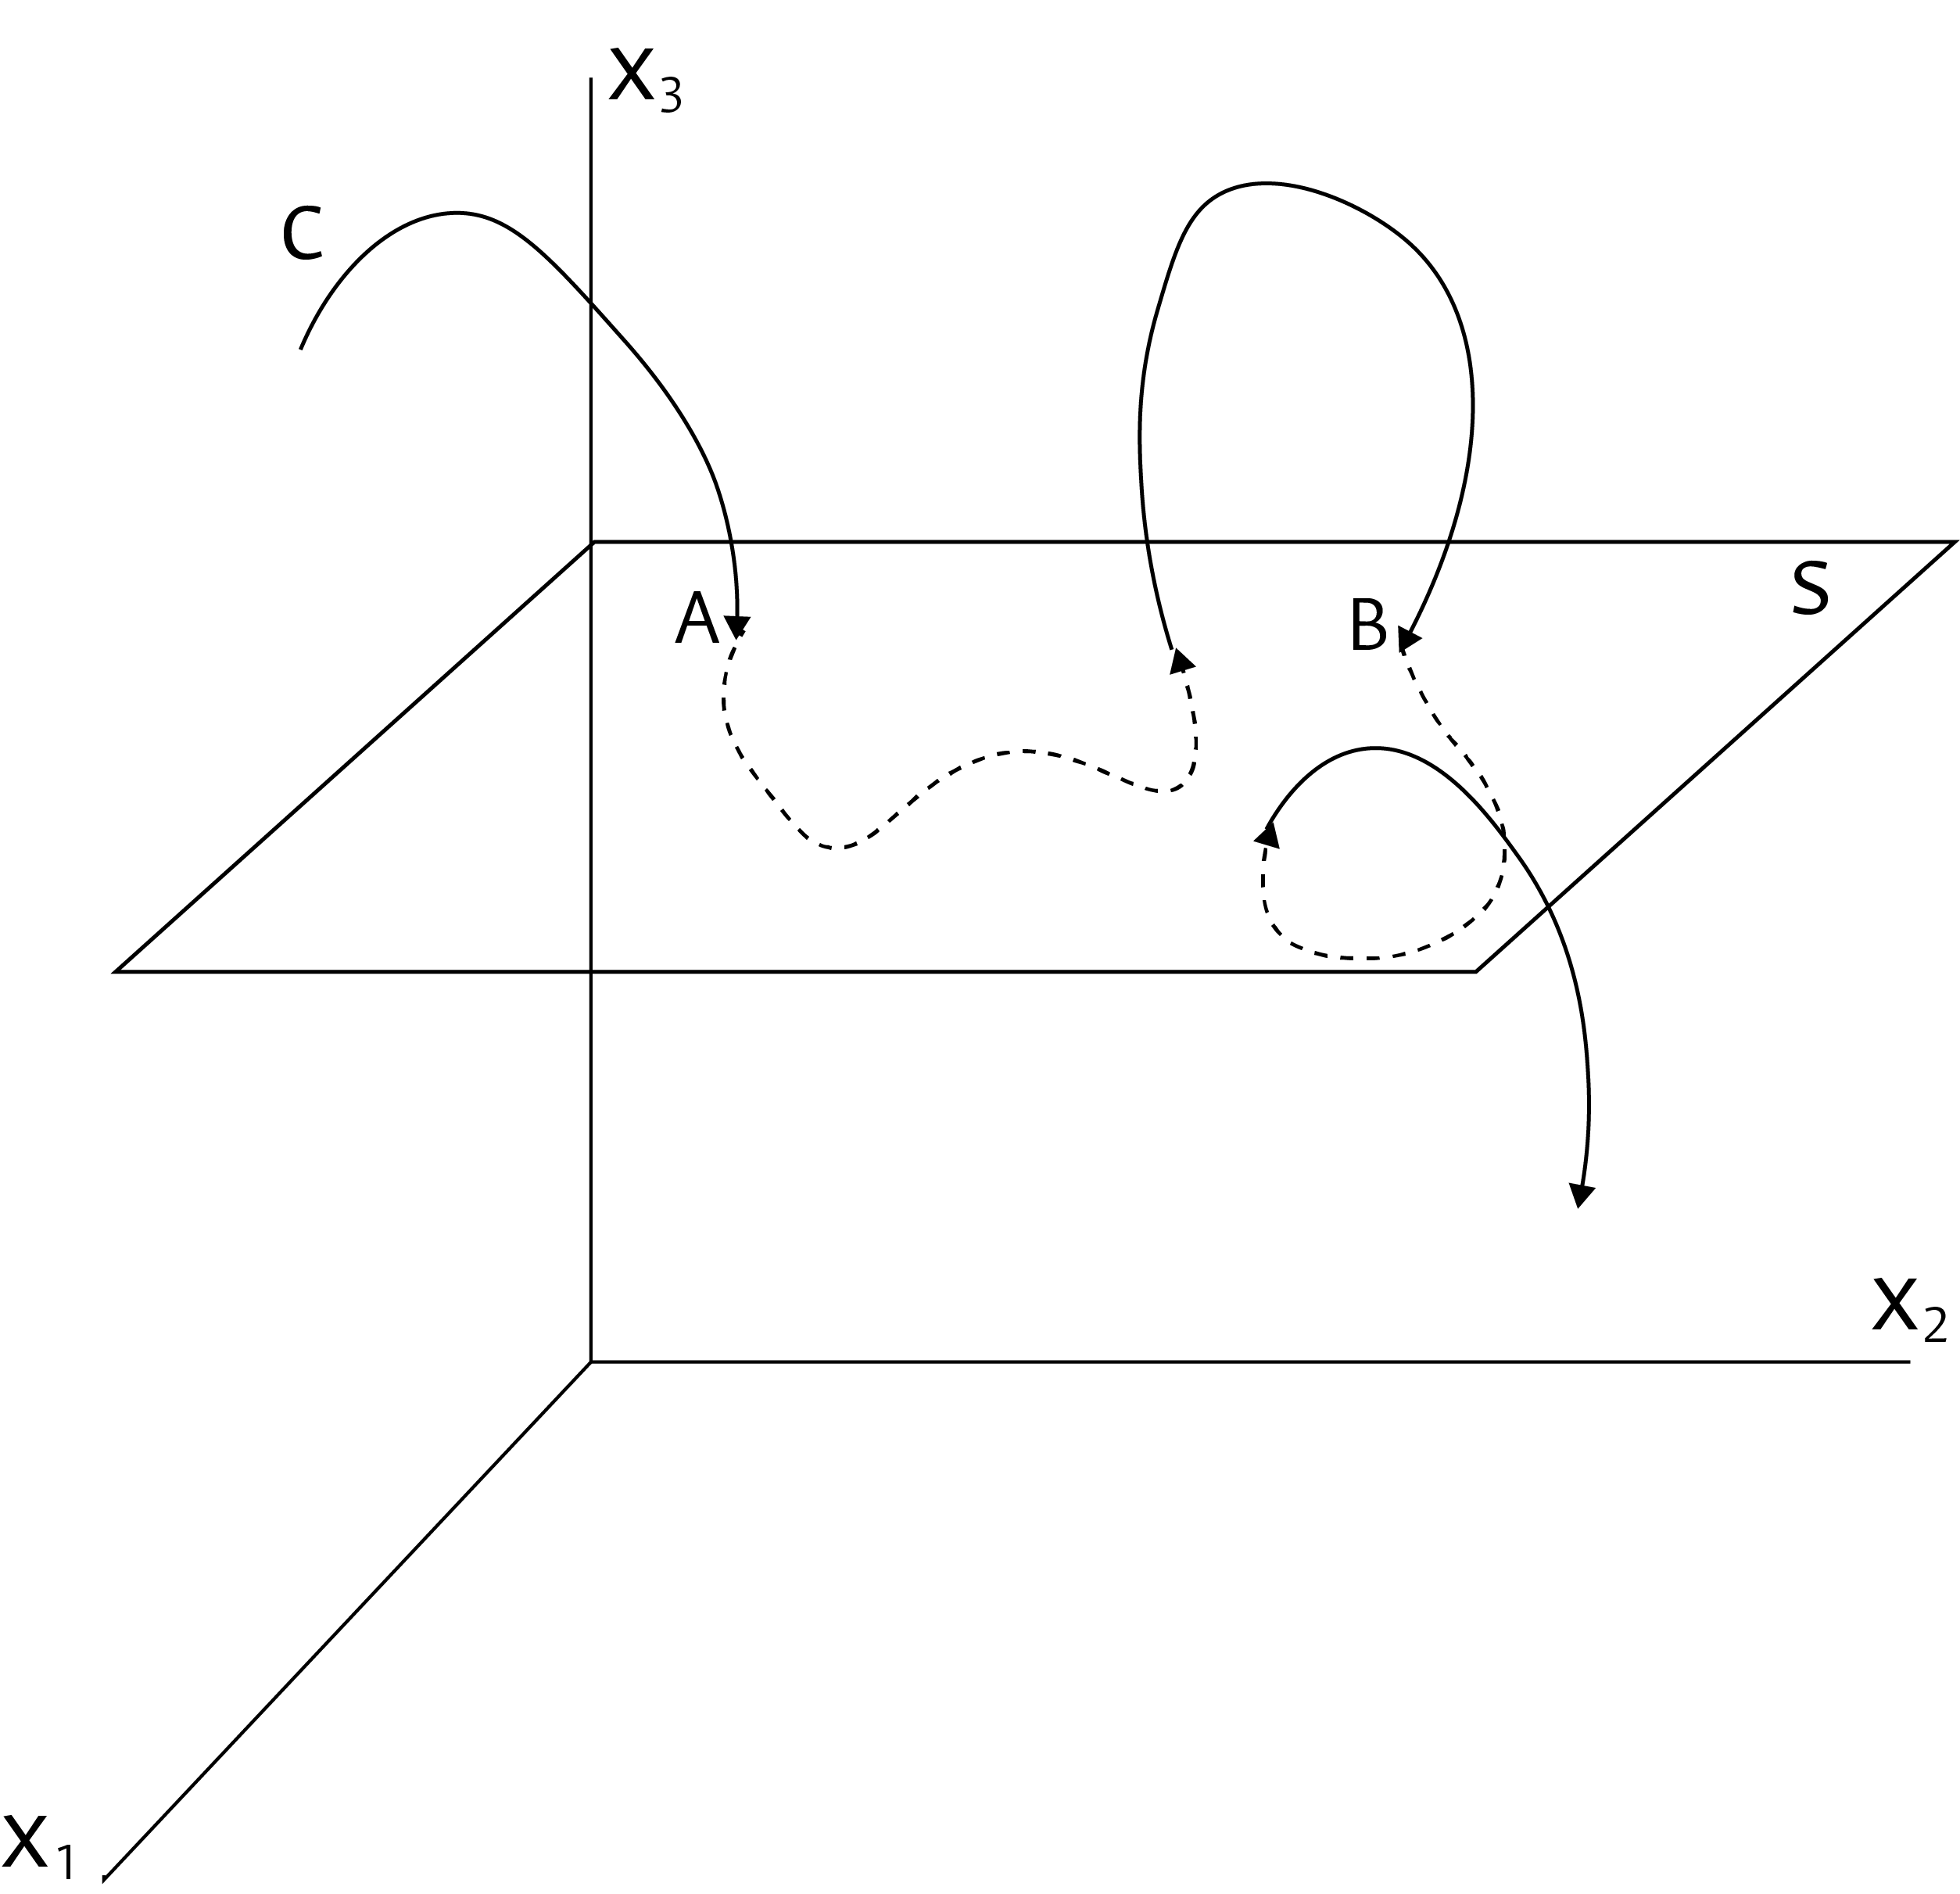
\includegraphics[width=10cm]{Figures/poincare_scheme.png}
\caption{Poincaré section on a two dimensional plane}
\label{fig:poincare_scheme}
\end{figure}

Fig (\ref{fig:poincare_scheme}) shows a Poincaré section on a two dimensional plane $S$ where the fixed condition will be $x^{3}=c$ where $c$ is a constant value. The points labeled as A and B represent the succesive intersections of the trajectory followed by the system with the plane $S$, this crossing is always considered to be on the same direction, a crossing of the plane through the opposite direction will result into another section. Given the point A, by using Equation (\ref{eq_:vect_diff_eqs}), we can certainly determine the position of point B, this is because A can be used as an initial condition to determine B. The same argument can be used to determine A given B as initial condition, this is done just by changing the sign of time on the same equation. Thus, the Poincaré map in this illustration represents an invertible two dimensional map that transforms the coordinates $(x_n^{(1)},x_n^{(2)})$ of the $n$th piercing of the surface section to the coordinates $(x_{n+1}^{(1)},x_{n+1}^{(2)})$ at piercing $n+1$. This map can be generalized to an $N$ dimensional flow with an $N-1$ dimensional invertible map.

\section{Hamilton equations and Symplectic Structure}

Hamiltonian systems are a class of dynamical systems that occur in a wide variety of circumstances, the special properties of Hamilton's equations of motion that are characteristic of this kind of systems endow Hamiltonian systems with attributes that differ qualitatively and fundamentally from other systems.\par 

The dynamics of a Hamiltonian system can be completely determined by a single function commonly known as the Hamiltonian, $H(\bm{p},\bm{q},t)$. The state of the system is specified by its \say{momentum} and \say{position} usually known as $\bm{p}$ and $\bm{q}$ respectively, both vectors with dimension $N$. $N$ is also known as the number of degrees of freedom of the system. Given the Hamilton's equations, the we can determine the trajectory  $(\bm{p}(t),\bm{q}(t))$ that the system follows in the $2N$ dimensional phase space, these equations are given by

\begin{equation}
\frac{d \bm{p}}{dt} =-\frac{\partial H(\bm{p},\bm{q},t)}{\partial \bm{q}},
\label{eq:pdot_hamil}
\end{equation}
\par 
\begin{equation}
\frac{d \bm{q}}{dt} =\frac{\partial H(\bm{p},\bm{q},t)}{\partial \bm{p}}.
\label{eq:qdot_hamil}
\end{equation}
In the special case where the Hamiltonian has no explicit time dependance, $H=H(\bm{p},\bm{q})$, given  Hamilton's equations of motion it can be deduced that as $\bm{p}$ and $\bm{q}$ vary with time, the value of $H(\bm{p}(t),\bm{q}(t))$ remains constant:
\begin{equation*}
\frac{dH}{dt}=\frac{d\bm{q}}{dt}\frac{\partial H(\bm{p},\bm{q})}{d\bm{q}}+\frac{d\bm{p}}{dt}\frac{\partial H(\bm{p},\bm{q})}{d\bm{p}}=\frac{\partial H(\bm{p},\bm{q})}{d\bm{p}}\frac{\partial H(\bm{p},\bm{q})}{d\bm{q}}-\frac{\partial H(\bm{p},\bm{q})}{d\bm{q}}\frac{\partial H(\bm{p},\bm{q})}{d\bm{p}}=0
\end{equation*}
Thus if we identify the value of the Hamiltonian as the energy $E$ of the system, we conclude that the energy is conserved in the case of time independent systems, $E=H(\bm{p},\bm{q})=constant$ \cite{ott_chaos_2002}.\par

Another interesting feature of Hamilton equations and Hamiltonian systems is that we can write Equations (\ref{eq:pdot_hamil},   \ref{eq:qdot_hamil}) in matrix form as
\begin{equation}
\frac{d\tilde{\bm{x}}}{dt}=\bm{F}(\tilde{\bm{x}},t),
\label{eq:symplectic1}
\end{equation}
by taking $\tilde{\bm{x}}$ to be the $2N$ dimensional vector
\begin{equation}
\tilde{\bm{x}}=\begin{pmatrix}
\bm{p}\\
\bm{q}
\end{pmatrix},
\end{equation}
and by taking $\bm{F}(\tilde{\bm{x}},t)$ to be 
\begin{equation}
\bm{F}(\tilde{\bm{x}},t)=\bm{S}_N \cdot \frac{\partial H}{\partial \tilde{\bm{x}}},
\label{eq:symplectic2}
\end{equation}
where $\bm{S}_N$ is the so called symplectic matrix given by 
\begin{equation}
\bm{S}_N=
\begin{bmatrix}
\bm{O}_N & -\bm{I}_N \\
\bm{I}_N & \bm{O}_N
\end{bmatrix}
\label{eq:symplectic_matrix}
\end{equation}
where $\bm{I}_N$ is the $N$ dimensional identity matrix, $\bm{O}_N$ is the $N \times N$ matrix of zeros, and
\begin{equation}
\frac{\partial H}{\partial \tilde{\bm{x}}}=\begin{bmatrix}
\partial H / \partial \bm{p} \\
\partial H / \partial \bm{q}
\end{bmatrix}.
\label{eq:sympl_hamil}
\end{equation}
From this vector notation we see how restricted the class of Hamiltonian systems is. In particular, a general system described as the form of (\ref{eq:symplectic1}) necessarily requires for the specification of all of the components of the vector function $\bm{F}(\tilde{\bm{x}},t)$ being used, while by (\ref{eq:symplectic2}), if the system is Hamiltonian, it is specified uniquely by a single scalar function of $\bm{p}$, $\bm{q}$ and $t$ which corresponds to the Hamiltonian.\par

One of the basic properties and a very important one of Hamilton's equations is that they preserve $2N$ dimensional volume in phase space. This follows by taking the divergence of $\bm{F}(\tilde{\bm{x}})$ in Equation (\ref{eq:symplectic1}), which gives
\begin{equation}
\nabla \cdot \bm{F}=\frac{\partial}{\partial \tilde{\bm{x}}}\cdot \bm{F}=\frac{\partial}{\partial \bm{p}}\Bigg(-\frac{\partial H}{\partial \bm{q}}\Bigg)+\frac{\partial}{\partial \bm{q}}\cdot \Bigg(\frac{\partial H}{\partial \bm{p}}\Bigg)=0
\end{equation}
Thus, if we consider an initial closed surface $S_0$ in the $2N$ dimensional phase space and evolve each point that makes up the volume forward in time, we obtain at each instant of time $t$ a new closed surface $S_t$ which contains within it precisely the same $2N$ dimensional volume as the initial surface $S_0$. This follows as

\begin{equation}
\frac{d}{dt}\int_{S_t}d^{2N}\tilde{\bm{x}}= \oint_{S_t}\frac{d\tilde{\bm{x}}}{dt}\cdot d\bm{S}=\oint_{S_t}\bm{F}\cdot d\bm{S}=\int_{S_t}\frac{\partial }{\partial \tilde{\bm{x}}}\cdot d^{2N}\tilde{\bm{x}}=0,
\end{equation}
where the integrals $\int_{S_t} \cdots$ denote integration over the volume enclosed by $S_t$, $ \oint_{S_t}\cdots$ denotes a surface integral over the closed surface $S_t$, and the third equality is a consequence of applying the divergence theorem to the closed integral \cite{ott_chaos_2002}. From this result we can conclude that Hamiltonian systems do not posses what are called attractors in phase space. This incompressibility of phase space volumes for Hamiltonian systems is called Liouville's theorem \cite{ott_chaos_2002} \cite{goldstein2002classical}.\par

Perhaps we can say that the most important basic structural property of Hamilton's equations is that they follow a symplectic structure \cite{ott_chaos_2002}:
\begin{equation}
\frac{d\tilde{\bm{x}}}{dt}=\bm{S}_N\cdot \frac{\partial H}{\partial \tilde{\bm{x}}}.
\end{equation}
We can illustrate this geometry with the following arguments, if we consider three orbits and take them as if they are infinitesimally displaced from each other, $(\bm{p}(t),\bm{q}(t))$, $(\bm{p}(t)+\delta \bm{p}(t),\bm{q}(t)+\delta \bm{q}(t))$ and $(\bm{p}(t)+\delta \bm{p}'(t),\bm{q}(t)+\delta \bm{q}'(t))$, where $\delta \bm{p}$, $\delta \bm{q}$, $\delta \bm{p}'$ and $\delta \bm{q}'$ are infinitesimal $N$ vectors, then the quantity represented by
\begin{equation}
\delta \bm{p}\cdot \delta \bm{q}'-\delta \bm{q}\cdot \delta \bm{p}',
\end{equation}
which is to be called the differential symplectic area, will posses the characteristic to be independent of time,
\begin{equation}
\frac{d}{dt}(\delta\bm{p}\cdot\delta\bm{q}'-\delta\bm{q}\cdot\delta\bm{p}')=0.
\label{eq:sympl_area_no_time}
\end{equation}
The differential symplectic area may also be written in vector notation as
\begin{equation}
\delta\bm{p}\cdot\delta\bm{q}'-\delta\bm{q}\cdot\delta\bm{p}'=\delta\tilde{\bm{x}}^{\dagger}\cdot\bm{S}_N\cdot \delta \tilde{\bm{x}}',
\label{eq:sympl_area_matrix}
\end{equation}
where $\dagger$ denotes transpose.\par

To derive the equality given by (\ref{eq:sympl_area_no_time}) we may differentiate (\ref{eq:sympl_area_matrix}) with respect to time and make use of the Equations (\ref{eq:symplectic1}) - (\ref{eq:sympl_hamil}):

\begin{align}
\frac{d}{dt}(\delta \tilde{\bm{x}}^{\dagger}\cdot \bm{S}_N\cdot \delta \tilde{\bm{x}}')
&= \frac{d\delta \tilde{\bm{x}}^{\dagger}}{dt}\cdot \bm{S}_N\cdot \delta \tilde{\bm{x}}'+\delta \tilde{\bm{x}}^{\dagger}\cdot \bm{S}_N\cdot \frac{d\delta \tilde{\bm{x}}'}{dt}
\nonumber \\
&= \bigg(\frac{\partial \bm{F}}{\partial \tilde{\bm{x}}}\cdot \delta \tilde{\bm{x}}\bigg)^{\dagger}\cdot \bm{S}_N\cdot \delta \tilde{\bm{x}}'+\delta \tilde{\bm{x}}^{\dagger}\cdot \bm{S}_N \cdot \frac{\partial \bm{F}}{\partial \tilde{\bm{x}}}\cdot \delta \tilde{\bm{x}}'
 \nonumber \\
&= \delta \tilde{\bm{x}}^{\dagger}\cdot \Bigg[\bigg(\frac{\partial \bm{F}}{\partial \tilde{\bm{x}}}\bigg)^{\dagger}\cdot\bm{S}_N+\bm{S}_N\cdot \frac{\partial \bm{F}}{\partial \tilde{\bm{x}}}\Bigg]\cdot \delta\tilde{\bm{x}}'
\nonumber \\
&= \delta\tilde{\bm{x}}^{\dagger}\cdot\Bigg[\bigg(\bm{S}_N\cdot\frac{\partial^2 H}{\partial \tilde{\bm{x}} \partial \tilde{\bm{x}}}\bigg)^{\dagger}\cdot \bm{S}_N+\bm{S}_N\cdot\bm{S}_N\cdot\frac{\partial^2 H}{\partial\tilde{\bm{x}}\partial\tilde{\bm{x}}}\Bigg]\cdot\delta\tilde{\bm{x}}' \nonumber \\
&= \delta\tilde{\bm{x}}^{\dagger}\cdot\Bigg[\bigg(\frac{\partial^2 H}{\partial \tilde{\bm{x}} \partial \tilde{\bm{x}}}\bigg)^{\dagger}\cdot\bm{S}_N^{\dagger}\cdot \bm{S}_N+\bm{S}_N\cdot\bm{S}_N\cdot\frac{\partial^2 H}{\partial\tilde{\bm{x}}\partial\tilde{\bm{x}}}\Bigg]\cdot\delta\tilde{\bm{x}}' \nonumber \\
&=0,
\label{eq:proff_sympl_area}
\end{align} 
where we have used the properties of the symplectic matrix $\bm{S}_N\cdot\bm{S}_N=-\bm{I}_{2N}$ (where $\bm{I}_{2N}$ is the $2N$ dimensional identity matrix), $\bm{S}_N^{\dagger}=-\bm{S}_N$ and noted that $\partial^2H/\partial\tilde{\bm{x}}\partial\tilde{\bm{x}}$ is a symmetric matrix. We can also prove that the symplectic matrix $\bm{S}_N$ satisfies the following conditions \cite{arnold1968probemes} :
\begin{equation}
\bm{S}_N^{-1}=\bm{S}_N^{\dagger}=-\bm{S}_N
\end{equation}
and
\begin{equation}
\det(\bm{S}_N)=1,
\end{equation}
which can be obtained directly from Equation (\ref{eq:symplectic_matrix}).\par

Symplectic systems present a wide variety of mathematical properties \cite{arnold1968probemes}, but the one that is more relevant for this work, is that they conserve the volume on the $2N$ dimensional phase space, this means that symplectic dynamical systems follow the Liouville Theorem \cite{ott_chaos_2002}.\par

The fact that a Hamiltonian system conserves volume in the phase space has some consequences, we will highlight here the Poincaré Recurrence Theorem \cite{zaslavsky2005hamiltonian} \cite{zaslavsky2007physics}. When considering the movement of the system in a limited region of the phase space, which we denote as $\Gamma$, if we define a small area $A$ within this region (REF FIGURA QUE NO HE HECHO), with volume $\Gamma_A < \Gamma$, we can obtain a set of time values $\{ t_j\}$ for which the flow crosses this region from the inside out. The time intervals
\begin{equation}
\tau_j=t_{j+1}-t_j;\qquad j=0,1,2,...
\end{equation}
are the Poincaré Cycles and $t_j$ the Poincaré Recurrence Times. \par



FIGURA QUE NO HE HECHO DE LA REFERENCIA DE LOS CICLOS DE POINCARE\par

Poincaré proved that for a movement in a finite region of space in which the volume is preserved, the entire path should return to a previously determined region (for example $A$ in Figure FIGURA QUE NO HE HECHO) in a finite time and an infinite number of times. An exception occurs only if $A$ is a zero dimension set \cite{zaslavsky2005hamiltonian} \cite{zaslavsky2007physics} \cite{xavier2015banhos}.\par 

Thus, in this chapter, some general properties of Hamiltonian dynamical systems have been described. This was made possible even without taking into account time evolution analysis of the systems, that is, their dynamics. In the coming sections, this question starts to gain space, focusing attention on some characteristics of its dynamics, more specifically when there is the presence of regular movement, chaos or a mixture of both.



\subsection{Integrability in Hamiltonian problems}
Another important topic related to Hamiltonian systems involves integrability, we will see in this subsection that integrability will naturally lead to the concept of chaos. As we have previously stated, in the case where the Hamiltonian of the system has no explicit time dependence, $H=H(\bm{p},\bm{q})$, we have showed that Hamilton's equations imply that the Hamiltonian does not change in time $dH/dt=0$ and the energy identified as the Hamiltonian $E=H(\bm{p},\bm{q})$ is thus a conserved quantity. Therefore, orbits with a given energy $E$ are restricted to lie on the $(2N-1)$ dimensional surface $E=H(\bm{p},\bm{q})$ as a consequence of the dimensionality reduction due to the energy being a constant in time. A function $f(\bm{p},\bm{q})$ is said to be a constant of motion of a system with Hamiltonian $H$ if this quantity does not change in time even if $\bm{p}$ and $\bm{q}$ do. More generally, if we differentiate the function $f(\bm{p},\bm{q})$ with respect to time, and assuming that there is no explicit time dependence for the Hamiltonian, if we make use of the Hamilton's equations we obtain that
\begin{equation}
\frac{df}{dt}=\frac{d\bm{p}}{dt}\cdot\frac{\partial f}{\partial \bm{p}}+\frac{d\bm{q}}{dt}\cdot\frac{\partial f}{\partial \bm{q}}= \frac{\partial H}{\partial \bm{p}}\cdot\frac{\partial f}{\partial \bm{q}}-\frac{\partial H}{\partial \bm{q}}\cdot\frac{\partial f}{\partial \bm{p}}=0
\end{equation}
We call the expression appearing on the right hand side of the second equality the Poisson bracket between  $f$ and $H$ \cite{goldstein2002classical}, and we shall abbreviate it as $\{F,h\}$. Using this definition, we can write a necessary a condition for a general function $f$ to be a constant of motion when the Hamiltonian does not depend on time \cite{zaslavsky2005hamiltonian}, for $f$ to be a constant of motion then its Poisson bracket with the Hamiltonian must be equal to zero:
\begin{equation}
\{ f,H\} =0.
\end{equation}
(We can show using this condition also that the Hamiltonian is correspondingly a constant of the motion since $\{H,H\}=0$.)\par

Liouville and Arnold showed that motion subject for a big family of Hamiltonians can be reduced to a Hamiltonian system written in action-angle coordinates and related the constant of motion to a criteria of integrability \cite{arnol2013mathematical}. For a system with $N$ degrees of freedom to be integrable, in this theoretical framework, it is necessary for the system to posses $N$ constants independent of motion $f_i(\bar{p},\bar{q})$\footnote{If a constant cannot be described as a function of others, then it is called \say{independent} \cite{ott_chaos_2002}}, with $i=1,2,...,N$ in such a way that
\begin{equation}
\{f_i,H\}=0
\label{eq:integrability_1}
\end{equation}
and 
\begin{equation}
\{f_i,f_j\}=\delta_{ij}
\label{eq:integrability_2}
\end{equation}
where $\delta_{ij}$ is the so called Kronecker delta \cite{zaslavsky2005hamiltonian}. To state it in another way, the vectors $\bm{v_i}$, defined by
\begin{equation}
\bm{v_i}=\nabla f_i,
\label{eq:integrability_3}
\end{equation}
where $\nabla=(\partial/\partial q_1,...,\partial/\partial q_N,\partial/\partial p_1,...,\partial/\partial p_N)$ is the nabla operator of phase space, must be linearly independent at all the points in phase space  \cite{goldstein2002classical}. If the conditions (\ref{eq:integrability_1})-(\ref{eq:integrability_3}) apply to any $i$ and $j$, then we say that the $N$ constants of motion are in involution.\par 

When an $N$-dimensional Hamiltonian system is integrable possesing $N$ independent constants of motion, the topology of the surface on which its trajectories evolve in phase space is restricted to an $N$ dimensional torus \cite{zaslavsky2005hamiltonian}. For the case $N=2$, an orbit over a torus is shown in Figure (\ref{fig:trajectory_torus})

\begin{figure}[H]
\centering
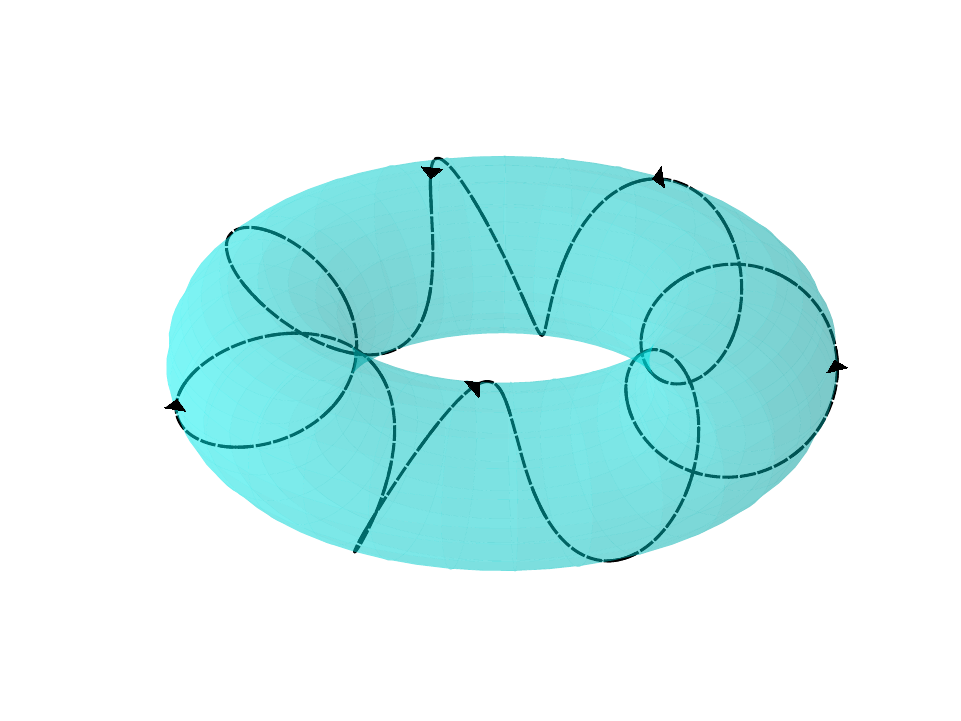
\includegraphics[width=0.7\textwidth]{Figures/trajectory_torus.png}
\caption{Trajectory on a torus for a bidimensional system with two constants of motion}
\label{fig:trajectory_torus}
\end{figure}

We can state a simpler description of the movement of integrable Hamiltonian systems over the $N$ dimensional torus by using the description in terms of the action-angle variables and the Hamilton-Jacobi equations, this formalism is explained in detail in Ref. \cite{goldstein2002classical}. 

When an integrable system begins to suffer the action of a disturbance of its trajectory, the tori whose ratio between frequencies is a rational or irrational number, behave in dfferent ways. The consequences of this disturbance on such tori are explained in detail by the KAM theorem


\subsubsection{KAM Theorem}
In the last subsections we introduced the necessary conditions for a system to be integrable. We also found that when we rewrite the Hamiltonian in terms of the constants of motion, especially in relation to the formalism of the angle-action variables, the system's movement can be described as to be limited to a rational or irrational $N$ dimensional torus, depending on the frequencies of the motion. But where does the integrability of a Hamiltonian system go? Or yet, what happens to rational and irrational tori when an integrable Hamiltonian system is subject to a disturbance? The answers to these questions came with the rigorous mathematical work of Kolmogorov, Arnold and Moser (KAM) and with the numerical studies developed on chaos and integrability after the advent of computer. The results obtained by Kolmogorov, Arnold and Moser became known as the KAM Theorem. The deduction of the theorem will not be detailed here, as it is ourside the scope of this work, only its results will be presented.\par

To describe the KAM theorem, we consider a disturbed Hamiltonian system, written in terms of the action-angle variables as
\begin{equation}
H(\bm{I},\bm{\theta})=H_0(\bm{I})+\epsilon H_1(\bm{I},\bm{\theta}),
\end{equation}
where $H_0(\bm{I})$ is the integrable Hamiltonian, $H_1(\bm{I},\bm{\theta})$ the perturbation and $(\bm{I},\bm{\theta})$ the action-angle variables of perturbed system.\par

The main idea of the KAM Theorem is to consider the effect of the disturbance on invariant Tori \footnote{A torus is called invariant if once the motion of the system starts on its surface, the motion will remain on it \cite{ott_chaos_2002}.} instead of the trajectories in the phase space \cite{zaslavsky2005hamiltonian}.



\subsubsection{Need of numerical algorithms}

The perturbation of the Hamiltonian leads to the system being difficult to integrate (even impossible in some cases) in terms of analytical solutions of the Hamilton equations of motion sometimes. For this reason numerical algorithms are very helpful in the way that they can describe the dynamics of the system step by step in an approximate way without the need of the analytical solutions, this will be our approach in this work. Choosing the correct numerical algorithm and its parameters so that it integrates a system of differential equations correctly is not a trivial task and is a very active research topic in applied mathematics. For Hamiltonian systems the numerical algorithms that must be used to solve Hamilton equations of motion need to conserve the properties and structure of this family of differential equations, for this topic we dedicated the next section of this work.



\section{Symplectic Integrator}
As we said previously, symplecticness is a very important property of the Hamiltonian systems, this feature is also present on numerical integration meaning that the need of symplectic integrators algorithms arises when trying to solve these type of problems with a good precision. Numerical integrators, generally speaking, are  numerical mappings of the differential equations, most of the times these mappings are nonsymplectic. Applying nonsymplectic algorithms to Hamiltonian problems tend to show solutions where the area in phase space is not conserved. We show this problem in Figure (\ref{fig:euler}) which illustrates this issue by taking the fundamental problem of the harmonic oscillator and integrating its equations of motion using the standard first order differential equation solver known as the Euler method (which is a nonsymplectic integrator) and also a first order symplectic algorithm known as the Verlet Leapfrog method\cite{verlet1967computer}  \cite{forest1990fourth}. The general problem of nonsymplectic algorithms and Hamiltonian problems is their tendency to not conserve the energy in time, we see this feature on Figure (\ref{fig:euler}) where the trajectory of the nonsymplectic algorithm drifts in time as a consequence of energy being transferred to the system due to numerical error.



\begin{figure}[H]%
    \centering
    \subfloat[Position dynamics]{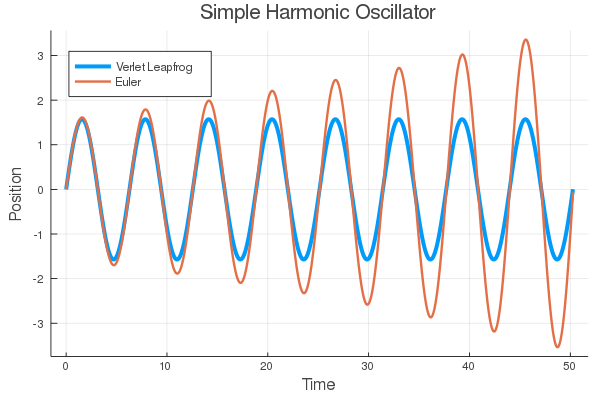
\includegraphics[width=10cm]{Figures/harmonic_oscillator.png} }%
    \qquad
    \subfloat[Phase space dynamics]{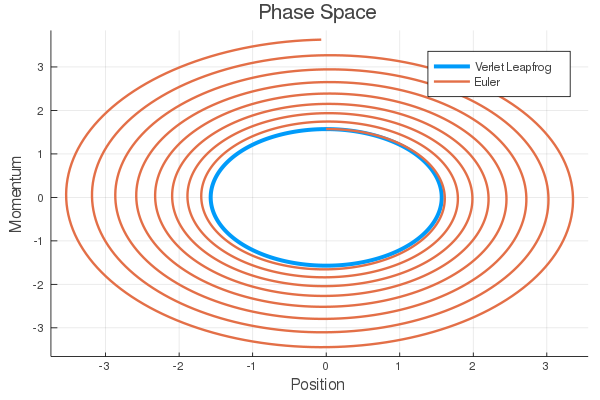
\includegraphics[width=10cm]{Figures/harmonic_oscillator_PS.png} }%
    \caption{Euler non symplectic integrator compared to symplectic Verlet Leapfrog method}%
    \label{fig:euler}%
\end{figure}

This failure of mimicking well known Hamiltonian dynamics suggested the consideration of schemes that generate a symplectic mapping $\Psi$ when applied to Hamiltonian problems, this mapping does not necessarily need to be perfect but at least really close to the symplectic manifold of the original problem. Such methods are called symplectic or canonical. Early references on symplectic integration are \cite{ruth1983canonical}\cite{channell1983symplectic}\cite{menyuk1984some}\cite{feng2010symplectic}\cite{kang1991symplectic}, but the first notions and ideas about the symplectic structure regarding integration techniques dates back to DeVogelaere in 1956 \cite{channell1990symplectic}.



\subsection{Importance of symplecticness in an integrator}
When talking about a domain $\Omega$ possesing a symplectic structure $\Lambda$, taking a smooth Hamiltonian function gives rise to a Hamiltonian system of differential equations known as the Hamilton equations. This domain we are talking about reffers to the phase space of the Hamiltonian system. If we consider a time step $h>0$, we can build a numerical scheme to solve these differential equations by using the function $\Psi :\Omega \rightarrow \Omega$ that depends on the step size $h$ and the Hamiltonian function of the system $H$. Then given an initial condition on the phase space $(p_0,q_o)$ we can estimate an aproximation to the solution at time $nh$ by iteratively applying the function $\Psi$
\begin{equation}
(p_{n+1},q_{n+1})=\Psi(p_{n},q_{n}).
\end{equation}
We may call the maping of the function $\Psi$ a symplectic integrator if the maping conserves the symplectic structure of a system, $\Psi \Lambda=\Lambda$\cite{markiewicz1999survey}\cite{de1956methods}\cite{ruth1983canonical} \cite{channell1983symplectic}.
A symplectic integrator is then an integrator whose solution resides on a symplectic manifold. Because of discretization error, when it is solving a Hamiltonian system it doesn't get exactly the correct trajectory on the manifold. Instead, that trajectory itself is perturbed by $\mathcal{O}(\Delta h^n)$ for the order $n$ from the true trajectory where $\Delta h$ is the timestep difference. Because of these arguments there is a linear drift due to numerical error of this trajectory over time. Normal integrators tend to have a quadratic (or more) drift, and do not have any good global guarantees about this phase space path, it only guarantees the path in a local sense.\par




Therefore symplectic integrators tend to capture the long-time patterns better than normal integrators because of this lack of drift in the trajectory and this almost guarantee the periodicity of certain problems at least for the desired time span. 

\subsection{Conservation of constants of motion}
As we have seen previously, when one uses a symplectic integrator of order $n$ what you do is to solve in an exact way the evolution of the system, but not using the Hamiltonian $H$ but one softly perturbated as $\tilde{H}=H+\epsilon H_1$, where $\epsilon=t^n$ and $H_1=H_1^0+hH_1^1+h^2H_1^2+...$ If what we really want to obtain is a qualitative information of the behavior of the system, we can expect that if $\epsilon H_1$ is sufficiently small, the system will evolve in a very similar way for $\tilde{H}$ as for $H$.\par

Consider now a system that has $m$ independent constants of motion $J_i$ where $i=1,...,m$, this means that for every $J_i$ it satisfies the condition of a null Poisson bracket with the Hamiltonian as $\{H,J_i\}=0$. As the integrator is solving in an exact way the evolution due to the Hamiltonian $\tilde{H}$, it will follow that the constants of motion, in general, will not be constant as they will not have a null Poisson bracket, in principle, with this new Hamiltonian. Nonetheless, the following is obtained
\begin{equation}
\{\tilde{H},J_i\}=\{H+\mathcal{O}(h^n),J_i\}=\mathcal{O}(h^n).
\end{equation}
Despite some exceptions, the constants of motion $J_i$ will not be constant along the evolution of the system, but they will disagree to being it in the same order as the energy does. Therefore, for an efficient integrator with high order precision the constants of motion will certainly be constant along the dynamical trajectory.

\subsection{Chaos and integrators}

Numerical chaos has been a very interactive branch of study for many years specially ever since numerical computations where able to be performed on computers . As we have shown, numerical stability of differential equations is very sensitive to systems involving chaos, even the slightest difference on the floating point error gives rise to diverging trajectories in phase space, this makes chaotic systems very interesting problems numerically speaking. As we know, floating numbers that computer algorithms work with have a finite value for decimals, when computing a solution of a differential equation using a given algorithm computers truncate this decimals leaving some round-off error. These truncations are not overseen by chaotic systems, chaotic systems have the nature of amplifying the slightest disturbance of the system into an observable result, this means that numerical truncations on floating point numbers have long term consequences when interpreting what we consider the solution. Therefore it is necessary to take into account these considerations regarding round-off precision when solving a chaotic system.\par

Numerical integrators and chaos consequently gather on an exotic dance of conditions to consider, on the one hand it is important for integrators to have a high order of accuracy by using intermediate steps before computing a definitive step on the trajectory of the solution and it is also important to have a small enough integration step to manage sensibility for the trajectory; on the other hand, error propagation of the floating point decimal truncation everytime the integrator performs an operation discourages all the effort put into calculating derivatives using intermediate steps and raises the question on what is the important aspect to consider. The answer is often unknown, solving these numerical problems with optimal efficiency is truly a very complicated task for the majority of chaotic problems\cite{lozi2013can}.\par 

Some chaotic problems might require calculations with a precision not always performed by usual codes and computers and if this is achieved the computational resources needed to arrive to a fixed point solution might be way to big to calculate \cite{galias2016numerical}.\par 

For the case of Hamiltonian systems, if the system is perturbed by a certain degree, the KAM theorem gives us information about the quasiperiodic orbits that will arise in the dynamics of the system\cite{arnold2009proof}\cite{kolmogorov1954conservation}\cite{tabor1989chaos}. If a normal Hamiltonian system is perturbed to a certain degree the problem may become non integrable in the sense of its orbits not easily represented by analytical functions, this is where numerical integrators play a huge role on determining the dynamics of these systems. Therefore correct numerical algorithms that map the Hamiltonian dynamics in a correct way in systems including chaos plays a very important role in the area of numerical differential equations problems. This means that symplectic algorithms to solve the differential equations for Hamiltonian systems with these properties arise as a very useful tool due to the conservation of the important quantities of the overall system.



\section{Randomness in classical and quantum mechanics}

Randomness and chaos share similarities physically speaking, they amplify any type of noise from the microscopical degrees of freedom and show them visible in the outcome of the dynamics of the systems. The idea to achieve true randomness on experiments or random number generators is a dream for many experimentalists, but the true situation is that most of the times, classically you can't have the perfect un-biased scenario of randomness. One great example is illustrated by Diaconis et al. \cite{diaconis2007dynamical} where very precise measurements and theroretical descriptions are applied to the commonly known random event of the coin toss. The outcome of this research is that for natural flips the result of the coin is biased to come up as started $51\%$ of the times. Another example of a physical method to come up with random numbers is related to optical chaos \cite{li2010all}\cite{li2016fully}, it has  has a high potential to physically produce high-speed random numbers due to its high bandwidth and large amplitude. A prototype of a high speed, real-time physical random bit generator based on a chaotic laser was built in 2013 \cite{wang20134}.\par


Determinism defined as the property of events to be determined completely by previously existing causes is an important concept concerning classical mechanics, given the equations of motion of a system, we know in an exact way the state of the system in a future time with arbitrary precision. Chaotic systems are very sensitive to small changes on the initial conditions and they are often missunderstood as random, but as we have previously described, chaotic systems do not exhibit random behavior in the sense that it can be at any place located in phase space but we have shown that it certainly remains conditioned by a certain degree to the motion on the KAM tori giving place to quasiperiodicity.\par 

Another important example of randomness in classical physics is present for example in fluid and molecular dynamics, where the numbers of degrees of freedom is of the order around Avogadro's number, due to this big number it is convenient to treat systems in a probabilistic way instead of following the dynamics of each of the particles that compose the system. This is therefore a randomness in the dynamics but given as a consequence of the choice to not follow explicitly each particle, one could say it is a randomness on purpose. This doesn't mean that these types of systems can't be described and simulated without a good accuracy, on the contrary, the methods to describe these types of systems are very sophisticated and a very interactive branch of research\cite{ghil2012topics}\cite{liu2008location}.

On the other hand, quantum mechanics seems to have fundamental randomness in its roots, measurements are regarded as probability measurements of the system to be in a determined state.  The Born's interpretation of the quantum mechanics of the wave function implies that we can count only on a probabilistic description of reality, therefore quantum mechanics is inherently probabilistic \cite{born1955statistical}. Randomness in quantum mechanics is also regarded to be due to the interaction of a measurement apparatus and an environment with the initial pure states. This is consistent and parallel to the modern way of intepretations of the collapse of the wave functions and the quantum measurements \cite{wheeler2014quantum} 	\cite{zurek2003decoherence}\cite{zurek2009quantum}.\par 

It is important for us to talk about the experiment to measure a spin component along a direction. If we take the $z$ component  as an example similar to the Stern-Gerlach experiment \cite{gerlach1922experimentelle}, in this experiment the particles before the measurement are regarded to be in a neutral state along the $z$ component, after the particles go through the inhomogeneous magnetic field the spin aligns along a direction of the $z$ component and gets deflected along this direction. The result of the experiment is seen in a screen where two clouds of particles are seen, one in the upper location and one in the lower one. The counts of particles on each cloud is the same in both cases, this translates as the probability of the particles to be aligned along certain direction is the same. Particles then have a completely random probability to the aligned along certain direction, this idea can be compared with the one of the coin toss, only two possible outcomes of the measurement. There is a big difference between both pictures besides one being classical and the other one quantum, it is that the coin toss is not truly random as it depends strongly on the initial conditions on how the coin toss is made meanwhile the spin measurement seems to be totally random as long as the particle is initially in a non-commuting state with the $z$ component of the spin. This idea is the one we are going to exploit on the next chapters and explore a little bit the grounds of the environment and its role of introducing bias to the outcome of the measurements.


